\documentclass[12pt]{article}
\usepackage[2419335]{easymcm}
\problem{B}
\usepackage{palatino}  % palatino是 COMAP 官方杂志采用的更好看的 Palatino 字体
\usepackage{pdfpages}
\usepackage{longtable}
\usepackage{tabu}
\usepackage{threeparttable}
\usepackage{listings}
\usepackage{paralist}
\graphicspath{{img/}}
 \let\itemize\compactitem
 \let\enditemize\endcompactitem

\newcommand{\upcite}[1]{\textsuperscript{\textsuperscript{\cite{#1}}}}
\title{Probability-Based Rescue Model for Submersibles}

\begin{document}

\begin{abstract}
\setlength{\parskip}{0pt}
More than a century after the sinking of the Titanic, on June 19th 2023, a tourist submersible carrying five people disappeared near its wreckage, losing contact with the outside world. Despite extensive searches, no trace of it was found. In today's era of popular underwater exploration and tourism, it is of great significance to develop methods for quickly and accurately predicting the location of missing submersibles to facilitate timely rescue operations and prevent such tragedies from recurring. This paper attempts to find a way to minimize the search and rescue time. 

We build \textbf{two main models: the location model and the searching model} to solve the problem. The location model predicts the position of the lost submersible and the searching model uses data provided by the location model to search for it. We also consider the equipment we need to prepare and how our model can be extrapolated to account for more complex situations.

Firstly, in the \textbf{location model}, we take many things into account, including the velocity of the current, the density of the water, the geography of the sea floor and the probability that the missing submersible suffers a propulsion loss. We also consider the survival instincts of people in the submersible. Uncertainty arises from the possibility of losing propulsion(\textbf{internal uncertainty}) and the complexity of the environment(\textbf{external uncertainty}). To lower external uncertainty, we advise the submersible to send its location and speed back to the host ship periodically. These numbers serve as a starting point in our model. 
% After comparing our predictions with the real position, we can conclude that the predictions are reasonable. The visualized results can be found in the category \textbf{Model Implementation}.

Then, in the \textbf{Prepare} stage of the problem, we evaluate different types of search and rescue equipment, dividing their costs into three parts: the cost of the equipment itself(availability), the cost of training personnel(usage) and the cost of storage and maintenance. Taking these costs into account, we decide to use \textbf{the portable sonar} in the searching process. For the process of salvaging submersibles, we equip the rescue vessel with mechanical arms and iron cages to secure the submersible awaiting rescue. Since the lost submersible is most likely deep in the ocean, we choose to use \textbf{submarine} equipped with the portable sonar to search for it underwater.

After that, in the \textbf{searching model}, The direction of the submarine movement \textbf{constantly changes} according to the current probability distribution calculated by the location model. We also take the accumulated search results into account by wiping the probability of the searched(and failed) regions to 0. 
% In our tests, the search proceeded quite smoothly.

Finally, in the \textbf{Extrapolate} stage of the problem, we put forward our solutions to expand our model. To account for other locations, we plan to \textbf{update our geographic data}, including the velocity of the current, the density of water and the geography of the sea floor. As for when the number of submersibles increases, we accordingly increase the number of searching submarines and associate the submarines with lost submersibles, turning this new situation into our original one. We also put forward another idea in the \textit{Future Work} section.

After constructing the model, we implement it with python code and achieve good results. Code tests prove the accuracy and efficiency of our model. Results can be seen in the \textit{Model Implementation} section. In addition, our model is easy to implement and extend. By changing a few parameters in our code, we can stimulate more conditions of different sea areas, proving its good universality.


\vspace{5pt}
\textbf{Keywords}: Submersible Rescue; Probability Density; Convolution and FFT; Dynamic Prediction; Kinetics in Ocean

\end{abstract}

\maketitle

\tableofcontents 


\section{Introduction}

\subsection{Problem Background}
People always have a great interest in sunken ships and jewels. To explore the mysteries of these wrecks, we need to build submersibles that can ensure the safety of personnel. Considering that submersibles may lose contact with the host ship at any time and sudden mechanical failures could lead to the loss of propulsion, we hope to design a method to better predict the location of the submersibles and initiate search and rescue operations as soon as possible.

However, changes in the submersible's location will continuously affect our predictions of its position, thereby altering the host ship's search trajectory for the submersible. We need to construct mathematical models to guide the host ship's course and the depth at which to deploy search for the submarine, in the context of constantly changing prediction results. Additionally, we must consider the cost of the search equipment and attempt to find a more economical solution.

\begin{figure}[H]
\centering
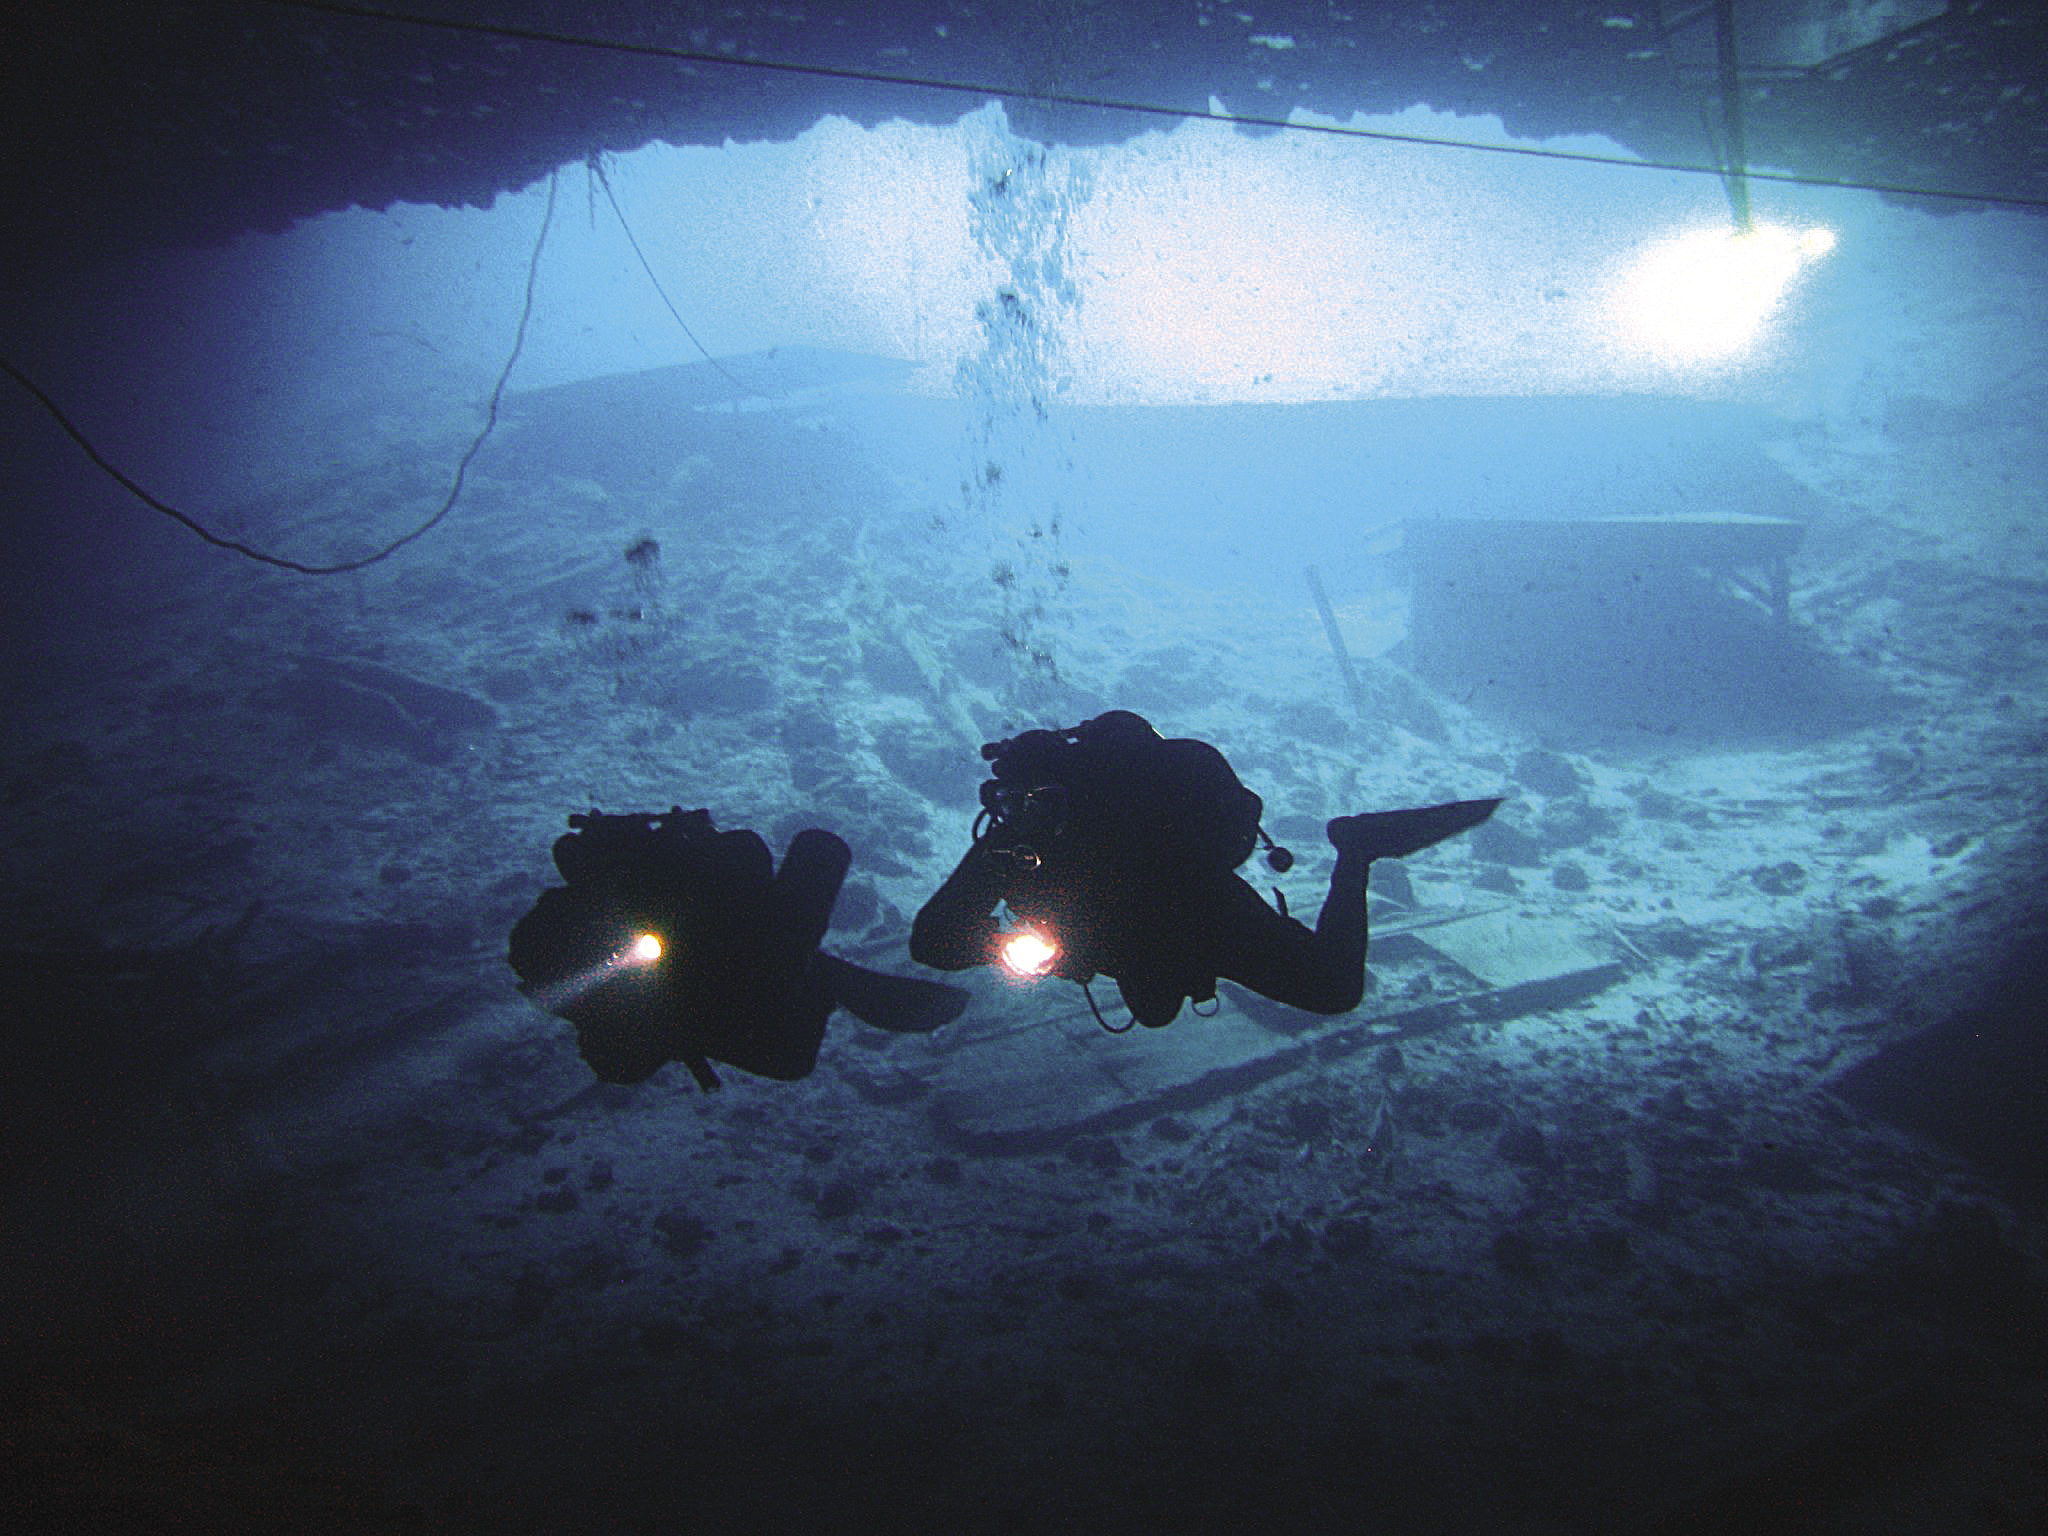
\includegraphics[width=.7\textwidth]{sunkenships.png}
\caption{Underwater Exploration of Sunken Ships}
\label{fig:Fire Situation}
\end{figure}

\subsection{Restatement of the Problem}
Considering the background information and the specific constraints given, the restatement of the problem can be expressed as follows:

\begin{itemize}
\setlength{\parsep}{0ex}
\setlength{\topsep}{2ex}
\setlength{\itemsep}{1ex}
\item Develop models to predict the submarine's location over time, addressing uncertainties in predictions. Identifying data the submarine can send to the host ship to reduce these uncertainties and specify the necessary equipment for this data transmission. 
\item Recommend additional search gear for the host ship, considering the costs associated with availability, maintenance and usage. 
\item Create a model to suggest initial deployment points and search patterns, aiming to minimize the time to locate a missing submersible. Adjust the likelihood of finding the submarine over time based on search efforts.
\item Consider how to adapt the model for other destinations like the Caribbean Sea and for tracking multiple submarines in the same area.
\end{itemize}

\subsection{Our Work}
The problem requires us to find a better way to locate the submersibles as quickly as we can:
\begin{enumerate}[\bfseries 1.]
    \setlength{\parsep}{0ex}
    \setlength{\topsep}{0.5pt}
    \setlength{\itemsep}{0.5pt}
    %\item Based on the accumulated search results, a prediction model of different kinds of parameters in the ocean is established;
    \item Based on the geographic data of the Ionian Sea and the information provided by the submersible before the loss of communication, a model to predict the \textbf{position of the submersible} is established;
    \item The \textbf{probability distribution of the location} of the submersible in the near future is acquired, and special cases such as the submersible experiencing mechanical failure after losing connection to the host ship are considered;
\item Based on the assumptions of the velocity and location, this article effectively demonstrates the \textbf{accuracy of our model}, as well as the timeliness of the rescue work.
\end{enumerate}
In order to avoid complicated description, and to intuitively reflect our work process, the structure of our work is shown in Figure \ref{fig:structure}:

\begin{figure}[H]
\centering
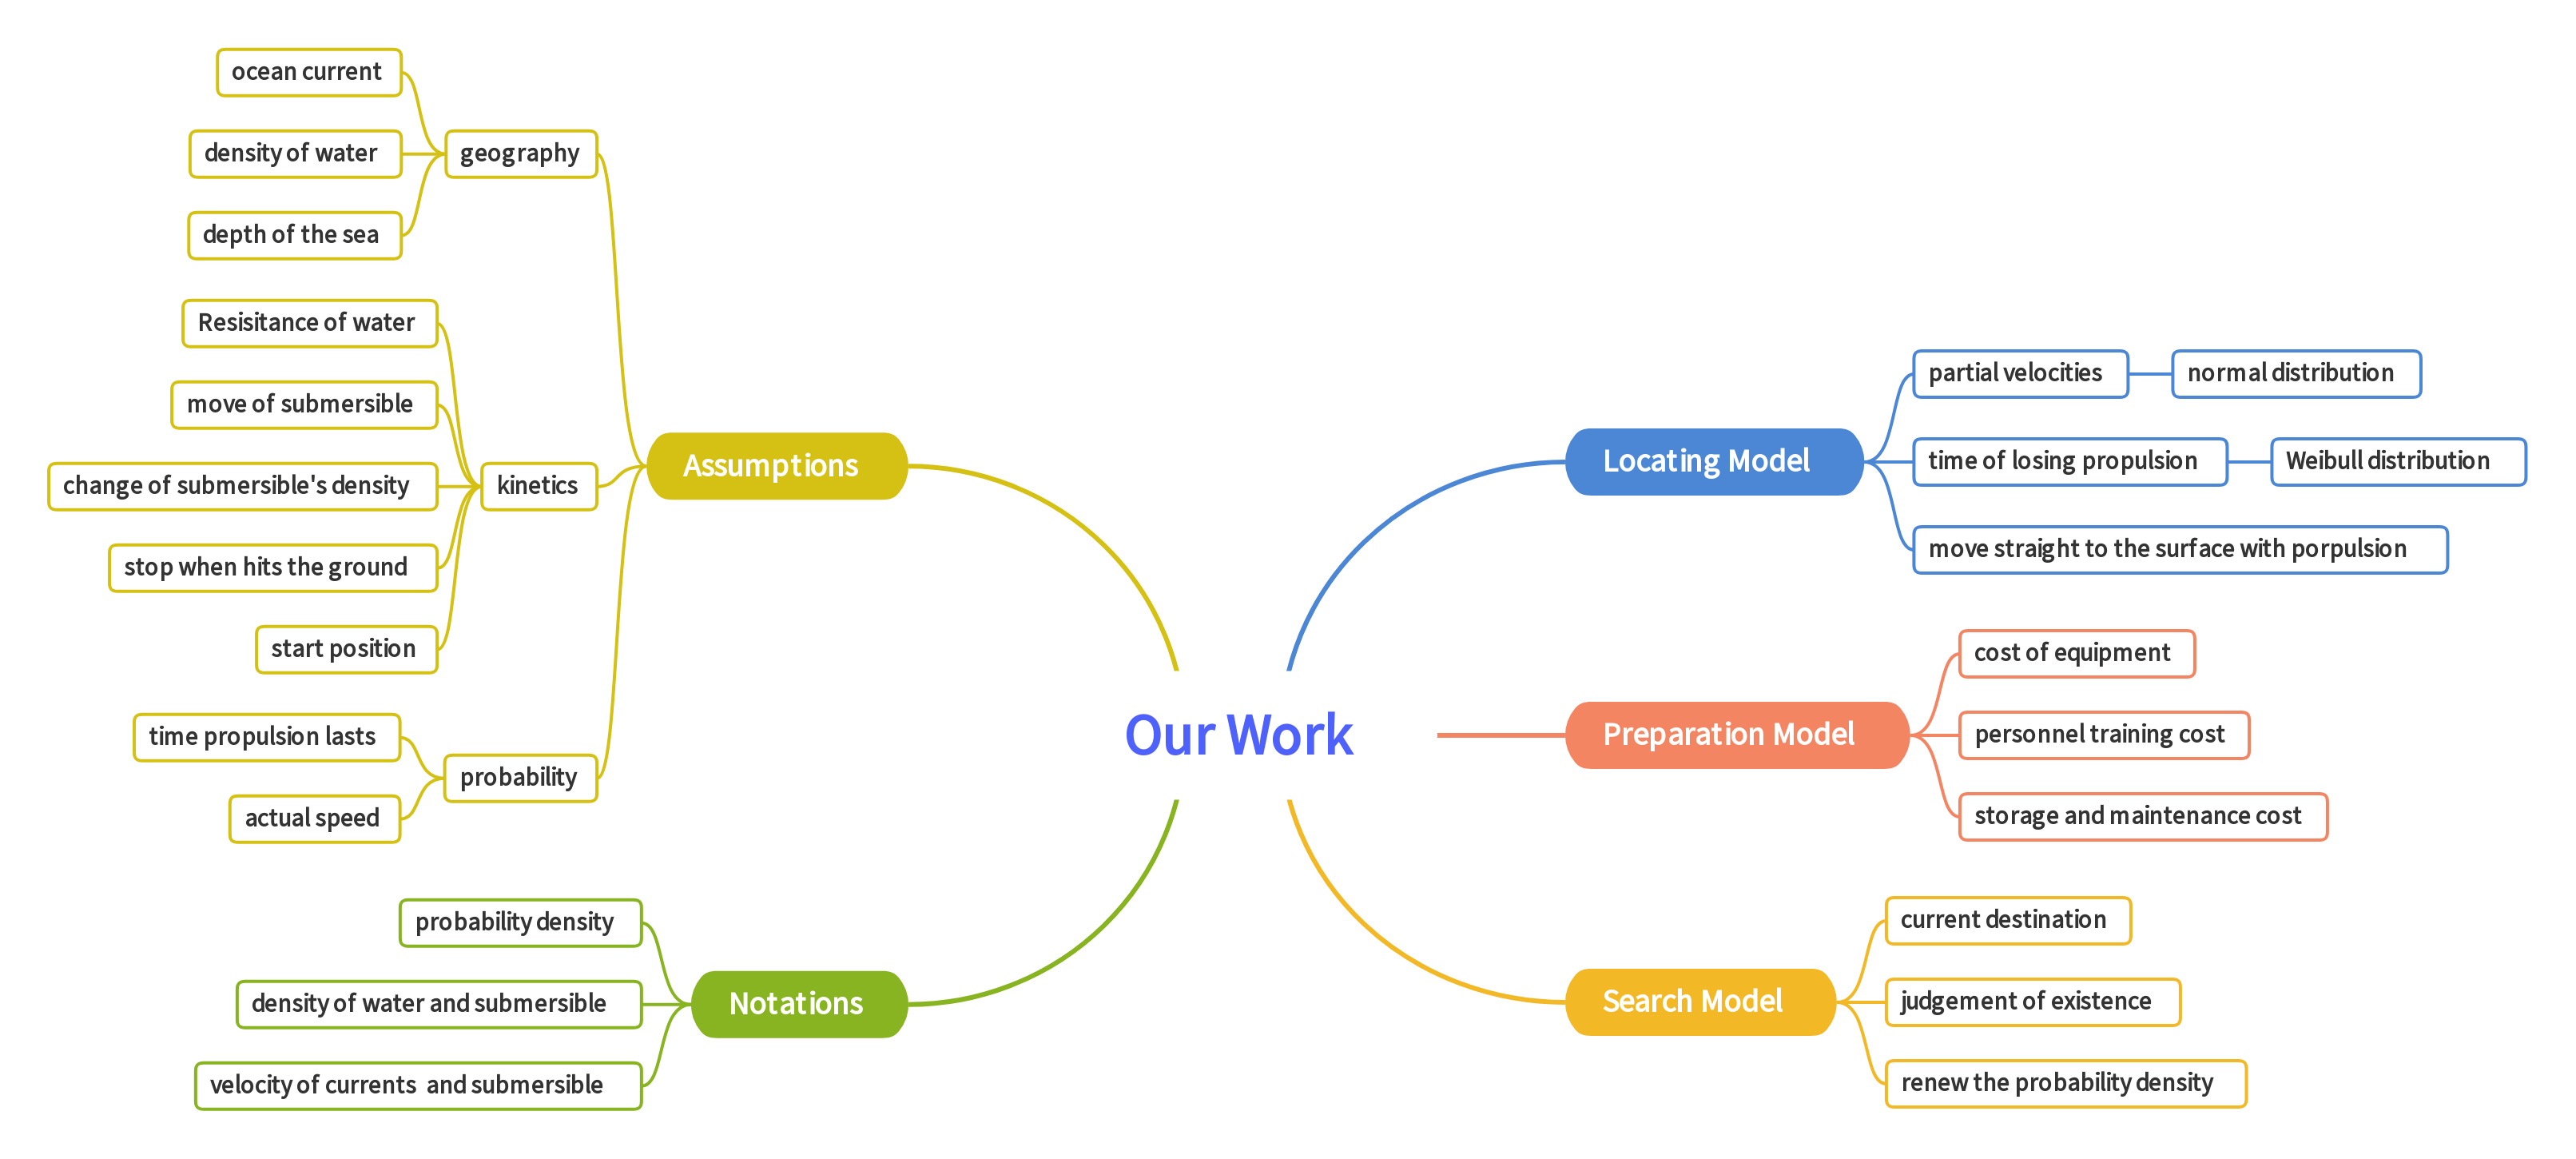
\includegraphics[width=\textwidth]{newmindmap.png}
\caption{Structure of Our Work}
\label{fig:structure}
\end{figure}
\vspace{-0.8cm}

\section{Assumptions and Explanations}
Considering the complex features of natural environment and the unpredictability of the submersible's precise speed, we have made a few reasonable assumptions to simplify the model beforehand. These assumptions fit into three categories, as shown below. Each hypothesis is closely followed by its corresponding explanation.
\subsection{Assumptions in terms of Geography}
\begin{enumerate}[\bfseries \textit{Assumption} 1:]
    %假设1:切块假设
    %\item \textbf{The Ionian Sea can be divided into definite regions, each with the same ocean current speed, the same water density and the same depth.}\\
    %There are countless points in the Sea, so it is impossible to calculate the probability of the submersible being on a particular coordinate. Therefore, to make it possible to acquire a probability distribution, we divide the Sea into regions with volume.Under the conditions above, when we move from one probability distribution to another, because we have already lost the information related to precise coordinates, we should use the same current speed, the same water density and the same depth. We realize that this isn't the real situation, but we still consider this assumption reasonable.
        %假设4:深度假设
	\item \textbf{The depth of the Ionian Sea at different horizontal positions is known.}
 
	The bathymetric data of the Ionian Sea can be accessed online, so we assume the depths of the Ionian Sea at different horizontal positions are known values.
        %假设3:海水密度假设
	\item \textbf{In the Ionian Sea, The density of water can be calculated.}
 
	The density of the water is mainly determined by two factors: temperature and salinity. Both of which can be accessed online. We use TEOS-10\cite{TEOS-10} to calculate the density of water.
	%假设2:洋流速度假设
    \item \textbf{In the Ionian Sea, the velocity of the ocean currents can be calculated.}\cite{Ionian Sea Research,Blue-greenway}
    
    In the framework of the EEA project BLUE-GREENWAY, ocean current conditions in the Ionian Sea have been studied for a period of ten years(2010-2019). There are already enough researches on the ocean currents, so we assume the velocity of the ocean currents can be calculated.
\end{enumerate}
\subsection{Assumptions in terms of Kinetics}
\begin{enumerate}[\bfseries \textit{Assumption} 1:]
    %假设1:阻力假设
    \item \textbf{Resistance is proportional to the relative velocity of the ship towards water.}
    
    The submersible will most likely experience resistance in the water. In our model, the flow resistance follows the equation $ F_x=-k\cdot\Delta v_x$. The same stands for y and z. Although this is not always the case, but compared to assuming resistance as a constant, what we use is usually a more accurate estimation.
    %假设2:时间微元假设
	%\item \textbf{We divide the time starting from the moment of communication lost into periods of 1s. In each period, velocity and force stays the same.}
 
	%The movement of the submersible is actually a three-dimensional kinetic problem. In our model, we solve this problem through the differential element method, with $ \Delta t=1s$. During this one second, velocity and force stays the same, meaning that acceleration stays the same as well. With the help of this assumption, we can determine the placement, velocity and acceleration one second later easily. If we do not make this assumption, we may have to solve some differential equations.
    %假设3:默认速度假设
	\item \textbf{From the moment that communication is lost, the submersible will move straight up with a given speed, until it is found or loses propulsion.}
 
	The rescuers wish to minimize the time of the location of the submersible. \textbf{So do the people in the submersible itself}. Under the belief that the shallower the submersible is, the easier the location work will be, if there is still propulsion after the loss of communication, the submersible will move straight up.
    %假设4:调整密度假设
    \item \textbf{From the moment that communication is lost, the submersible will change its density to a certain value.}
    
    Under the same belief in Assumption 3, people in the submersible will change the density of the submersible to a certain value below the density of normal water in order to go up.
    %假设5:速度归零假设
	\item \textbf{If at the end of a certain time period, the submersible touches the sea floor, its velocity will turn to zero.}
 
	There may be scenarios in which the submersible hits the sea floor. In real life, this is probably a non-perfect elastic collision between the submersible and the Earth. However, as we do not know the collision factor, we simply assume the collision to be completely inelastic. This is equivalent to changing the velocity to zero whenever a collision occurs.
    %假设6:搜救艇初位置假设
	\item \textbf{The searching submarine will be positioned at a fixed position at the beginning.}
 
	Taking maintenance costs into account, the searching submarine cannot be at sea all the time, waiting for a rescue mission to appear. Thus, we assume that the searching submarine stays at shore most of the time. This includes the moment when the loss of communication occurs.
\end{enumerate}
\subsection{Assumptions in terms of Probability}
\begin{enumerate}[\bfseries \textit{Assumption} 1:]
    %假设1:失去动力概率假设
	\item \textbf{The time that propulsion lasts(starting from the moment of communication lost) follows an Weibull distribution.}
 
	As stated in the problem, the submersible may suffer a loss of propulsion.The Weibull distribution is used frequently in reliability engineering and failure analysis, according with our scenario nicely.
    %假设2:速度正态分布假设
	\item \textbf{The actual speed of the submersible follows a normal distribution with a expectation of the given or calculated speed.}
 
	\textbf{\textit{Explanation:}}Due to the complexity of movement in water, after all our calculations, the actual velocity is ultimately uncertain. Even the velocity data sent back before the communication loss may be inaccurate. However, odds are that our calculations are not far from the precise numbers. That is why we assume the actual speed of the submersible to follow a normal distribution of the given or calculated speed.
\end{enumerate}
%Additional assumptions are made to simplify analysis for individual sections. These assumptions will be discussed at the appropriate locations.
These assumptions may be mentioned below again at the appropriate locations. 

\section{Notations}
Some important mathematical notations used in this paper are listed in Table 1. 
\begin{table}[H]
\begin{center}
\caption{Notations used in this paper}
\begin{tabular}{c l}
\toprule[2pt]
\multicolumn{1}{m{3cm}}{\centering Symbol}
&\multicolumn{1}{m{8cm}}{\centering Description }\\
\midrule
$x,y,z$& Coordinates of a point in a Cartesian coordinate system \\
$D(D\subset \mathbb{R}^{3})$& The range in which we discuss the problem\\
$P(x,y,z,t)$& The predicted probability density of the lost submersible \\ 
$\rho(x,y,z)$& Density of sea water \\
$\rho$& Average density of the lost submersible \\
$\Vec{v}_{c}(x,y,z)$& Velocity of currents \\
$\vec{v}_{s}$& Velocity of the searching submarine \\
$I_{R}(x,y,z)$& Equals to 1 if $(x,y,z)$ is in $R$, 0 if not\\

\bottomrule[2pt]
\end{tabular}\label{tb:notation}
    \begin{tablenotes}
        \footnotesize
        \item[*] *There are some variables that are not listed here and will be discussed in detail in each section. %此处加入注释*信息
    \end{tablenotes}
\end{center}
\end{table}
\vspace{-1cm}%在\end{table}下加一行\vspace{-1cm} 其中-1的作用是缩短与下方文字距离的

\section{Model Preparation}
In our model, we need some data such as the geography of the target sea area, the velocity of currents, etc.

\subsection{Data Collection}
The geography of the target sea area, that's to say the bathymetric data, and the temperature and salinity data can be accessed online. The temperature and salinity data are used to calculate the density of sea water.

Here are the database websites we can access data.
\begin{table}[H]
\begin{center}
\caption{Data and Database Websites}
\resizebox{\textwidth}{!}
{\begin{tabular}{c c}
\toprule[2pt]
\multicolumn{1}{m{5cm}}{\centering \textbf{Database Names}}
&\multicolumn{1}{m{10cm}}{\centering \textbf{Database Websites} }\\ %m后面是列宽
\midrule
Bathymetric Data & https://www.gebco.net/data\_and\_products/gridded\_bathymetry\_data/ \\
Temperature and Salinity Data & https://www.ncei.noaa.gov/products/world-ocean-database \\
\bottomrule[2pt]
\end{tabular}}
\end{center}
\end{table}

\begin{figure}[H]
\centering
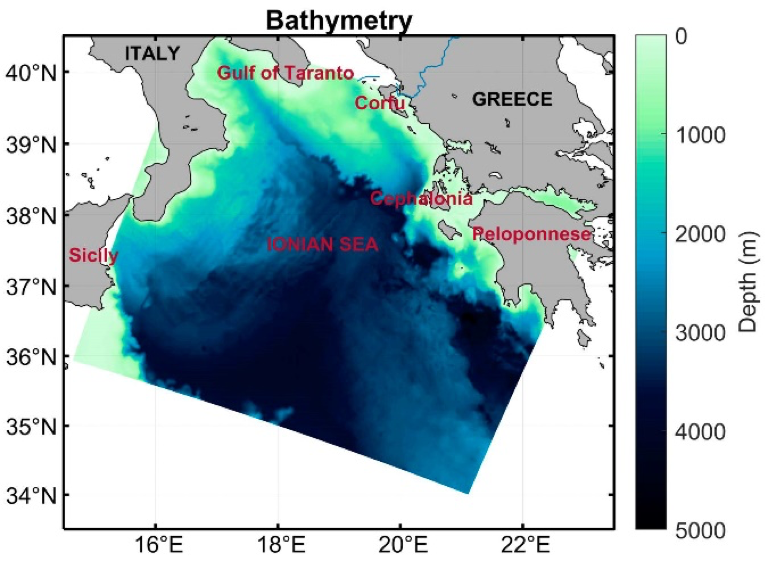
\includegraphics[width=.9\textwidth]{bathymetry.png} 
\caption{Bathymetry of the Ionian Sea\cite{Blue-greenway}}
\label{fig:Bathymetry}
\end{figure}
\vspace{-0.8cm}

\begin{figure}[H]
\centering
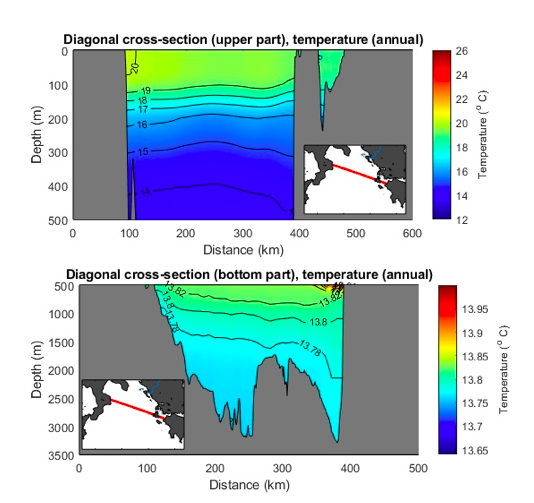
\includegraphics[width=.9\textwidth]{temperature.png}
\caption{Mean annual values of temperature along depth\cite{Blue-greenway}}
\label{fig:Bathymetry}
\end{figure}
\vspace{-0.8cm}

\subsection{Data Computation}
The velocity of currents cannot be accessed directly online, and it changes over time. But we have methods to compute the velocity with data that can be accessed.  

The velocity of currents can be estimated through the method given by current papers\cite{Ionian Sea Research,Blue-greenway}, which we won't discuss in detail.

\begin{figure}[H]
\centering
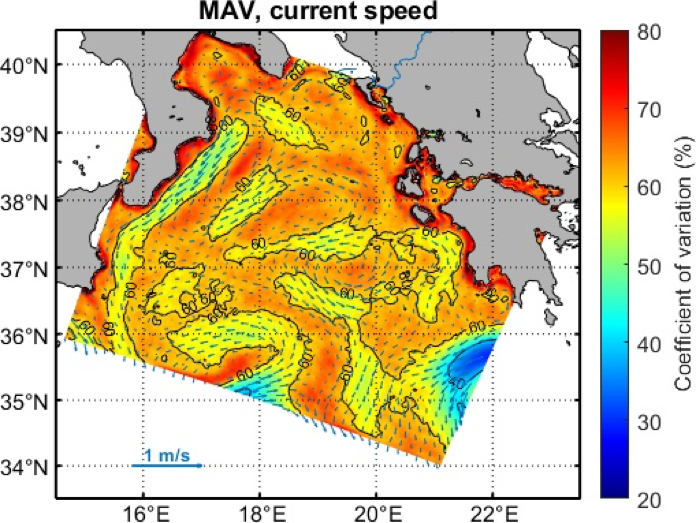
\includegraphics[width=.9\textwidth]{current speed.png}
\caption{Mean annual variability of surface current speed\cite{Blue-greenway}}
\label{fig:Bathymetry}
\end{figure}
\vspace{-0.8cm}

\section{Models}
\subsection{Location Model}
In this section, we will discuss our model of predicting the position of the lost submersible.
\subsubsection{Overall Introduction}
In the location model, we need to predict where the submersible is. 

Firstly, we assume that the submersible periodically sends its position to the host ship before communication loss. So we know when it is the time it loses communication. To achieve this, we may need some equipment like sonar system, VLF radio communication system, etc.\cite{communication methods}

We will consider many external factors to make our model as accurate as possible, Here is the factors our model takes into account: 

\begin{itemize}
    \item Probability that the submersible loses propulsion
    \item Different water density at different positions
    \item Impact from currents
    \item Geography of sea floor
    \item We argue that predicting submersible velocities to obey a certain distribution to model the effects of other external uncertainties.
\end{itemize}

Considering the complex of the outer environment, we do not just predict an exact position. Instead, we use probability density to represent the prediction of its position, which changes over time. 

See figure \ref{fig:heatmap}: A example of heatmap of probability distribution on a plane.

\begin{figure}[H]
\centering
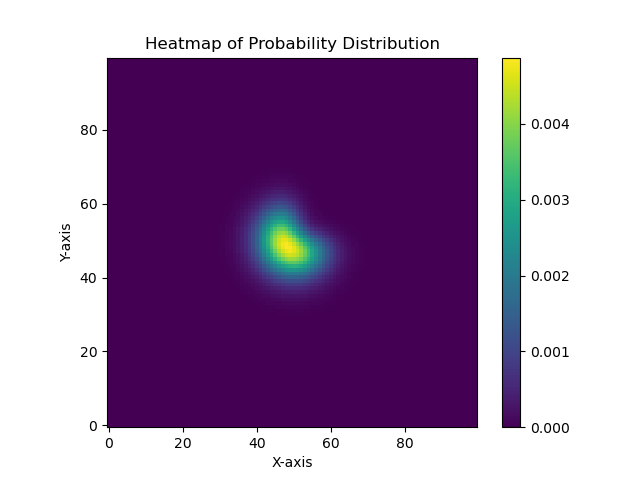
\includegraphics[width=.9\textwidth]{heatmap.png}
\caption{A probability distribution}
\label{fig:heatmap}
\end{figure}

To simulate the uncertainties of the external environment, we assume the predicted velocity is not a single value either. Instead, it obeys a normal distribution. And the average of the distribution is not a constant. It changes as the submersible is subjected to forces like gravity, buoyancy, as well as the thrust(or drag) by the currents.

Another important factor worth considering is the propulsion of the submersible. We can stipulate in advance that if its propulsion is not lost yet, then the submersible moves straight towards the surface, which is conducive to the rescue of the lost submersible as well as minimizing the cost of the rescue. Otherwise, when the propulsion is already lost, the submersible has to move by control of gravity, buoyancy and thrust(or drag) by the currents.
\subsubsection{Detailed Model Design}
Assume the probability of unit volume of the lost submersible being at $(x,y,z)$ is denoted by
$$P(x,y,z,t)$$
which can be initialized by the last information received from the submersible before loss of communication.

Assume the predicted velocity of the submersible is
$$\vec{v}=[v_{x},v_{y},v_{z}]^{T}$$

Considering the complex external environment, we assume the partial velocities in all directions follow a normal distribution(denoted as $\phi$), whose mean is respectively $v_{x}$, $v_{y}$, $v_{z}$.

The we can find the probability density after a short time by the formula below:
$$P(x,y,z,t+\Delta t)=\iiint_{D}P(u,v,w)\cdot \phi(x-u-v_{x}\cdot \Delta t)\cdot \phi(y-v-v_{y}\cdot \Delta t)\cdot \phi(z-w-v_{z}\cdot \Delta t)\cdot \mathrm{d}x\mathrm{d}y\mathrm{d}z$$

Then assume the probability that the submersible has lost propulsion is denoted by $p(t)$.

The Weibull distribution\cite{Weibull Distribution} is a commonly used probability distribution model for describing the reliability and lifetime distribution of systems. It particularly excels in characterizing the distribution of lifetimes for objects or systems. So we can assume the exact time when the submersible loses propulsion obeys a Weibull distribution. 

$$t_{0}\sim f(t;\lambda ,k)={\begin{cases}{\frac {k}{\lambda }}\left({\frac {t}{\lambda }}\right)^{k-1}e^{-(t/\lambda )^{k}},&t\geq 0,\\0,&t<0,\end{cases}}$$

See figure \ref{fig:Weibull distribution} for image of Weibull distribution.

\begin{figure}[H]
\centering
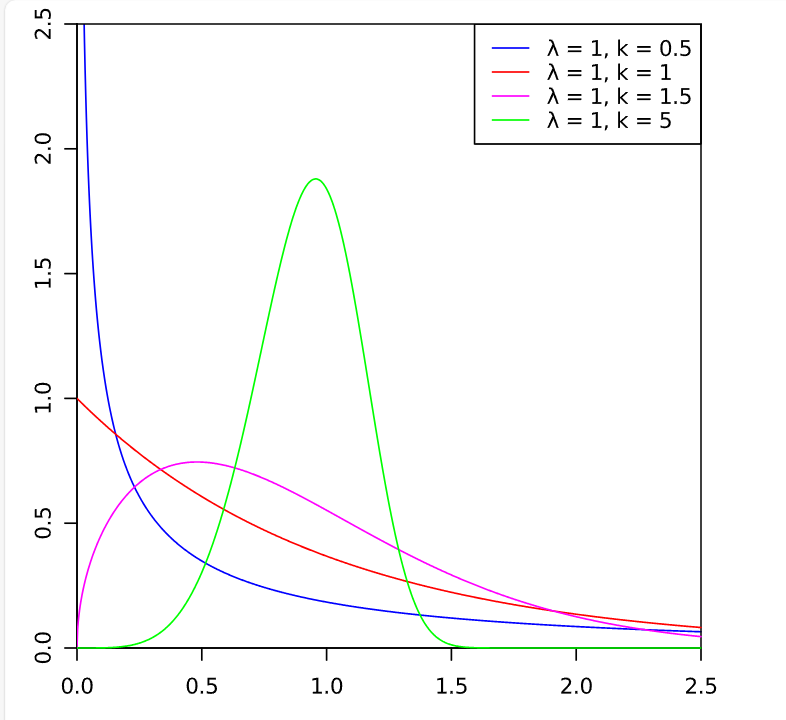
\includegraphics[width=.9\textwidth]{weibulldistribution.png}
\caption{Weibull distribution}
\label{fig:Weibull distribution}
\end{figure}

Then we can know
$$p(t)=\int_{0}^{t}f(s;\lambda,k)\mathrm{d}s=1-e^{-(t/\lambda)^{k}}$$

To facilitate the rescue and save costs, we stipulate that if the propulsion is not lost, then the submersible moves straight towards the surface at a constant speed. When the propulsion is lost, the submersible moves with currents and gravity. 

As we don't know whether the submersible has lost propulsion, we need to take both cases into account by their probabilities. Hence, we can calculate the velocity by the formula below:
$$\vec{v}(t+\Delta t)=\Vec{v_{0}}[1-p(t)]+[\vec{v}(t)+\Vec{a}(t)\Delta t]p(t)$$
where $\Vec{v_{0}}$ stands for the constant upward speed when propulsion remains, and $a(t)$ stands for the acceleration of the submersible when the propulsion is lost.

Now we focus on the acceleration of the submersible when the propulsion is lost. The forces on the submersible include buoyancy, gravity, and the thrust(or drag) of the current. 

The gravity and buoyancy can be easily found as below
$$G=mg=\rho gV \quad F_{b}=\rho_{0}gV$$
where $\rho$ stands for the density of the submersible.

As every position has different density of sea water and we don't know the exact position of the submersible, so we use a specially chosen value $\rho_{0}$ to represent the different value of water density. We choose $\rho_{0}$ as the weighted average according to probability. That is
$$\rho_{0}(t)=\iiint_{D}\rho(x,y,z)P(x,y,z,t)\mathrm{d}x\mathrm{d}y\mathrm{d}z$$
Here, $\rho(x,y,z)$ stands for the density of the water at position $(x,y,z)$, and we use TEOS-10 to find $\rho(x,y,z)$. TEOS-10(Thermodynamic Equation of Seawater - 2010) is the international standard for the use and calculation of the thermodynamic properties of seawater.\cite{TEOS-10}

Then comes the thrust(or drag) of the currents, which is related to the velocity of the currents. We can assume the force by currents is proportional to the velocity difference, that is
$$\Vec{F}=k(\Vec{v}_{s}-\vec{v})$$

The way we choose $\Vec{v}_{s}$ is the same as how we choose $\rho_{0}$. We choose the special current velocity(to represent different values of currents' velocity) $\Vec{v}_{s}$ by
$$\vec{v}_{s}(t)=\iiint_{D}\Vec{v}_{c}(x,y,z)P(x,y,z,t)\mathrm{d}x\mathrm{d}y\mathrm{d}z$$
Here, $\Vec{v}_{c}(x,y,z)$ stands for the velocity of the currents at position $(x,y,z)$, and we can calculate $\Vec{v}_{c}(x,y,z)$ as mentioned in \textbf{Data Computation} section.

Then we have 
$$m\vec{a}=\Vec{F}+[0,0,G-F_{b}]^{T}$$
From that we can find the accelerate and then find the velocity $\vec{v}(t+\Delta t)$.

Up to now we have considered different density of water, the probability of losing propulsion, and impacts of currents. Now we take the geography of the sea floor into account. When the submersible hits the sea floor, we can assume it loses velocity at once and it is not subject to horizontal force anymore as long as it doesn't leave sea floor.

\subsection{Preparation}
In this section, we will discuss our model on how to prepare, and the equipment to choose. To determine the equipment needed for search and rescue operations, we must consider the cost of various search and rescue devices. For any piece of equipment, the costs associated with completing a full search and rescue operation can be divided into three parts: equipment cost, personnel training cost, and storage and maintenance cost.

In the table listed below, we collect common search and rescue equipment available on the market and provided their prices(it is important to note that different models of search and rescue equipment and the region of purchase can affect their prices. For simplification, we use the prices in China and converted them into US dollars for calculation). All the data below are selected from China's major e-commerce platforms like alibaba and taobao, based on underwater sonar search requirements.

\begin{table}[H]

\begin{tabular}{|>{\centering\arraybackslash}p{0.2\linewidth}|>{\centering\arraybackslash}p{0.2\linewidth}|>{\centering\arraybackslash}p{0.2\linewidth}|>{\centering\arraybackslash}p{0.2\linewidth}|} \hline  
Equipment                           & Cost of Equipment & Personnel Training Cost & Storage and Maintenance Cost\\ \hline  
Portable Sonar                      & \$2000            & \$1000                  & \$500                   \\ \hline  
Deep-sea Camera                     & \$8000            & \$1500                  & \$800                   \\ \hline  
Search and Rescue Drones            & \$20000           & \$2000                  & \$1000                  \\ \hline  
Search and Rescue Underwater Robots & \$30000           & \$2500                  & \$1200                 
 \\ \hline \end{tabular}
\caption{Cost of Common Equipment}
\label{tab:my_table}
\end{table}

Considering the total cost, we choose the portable sonar, which will be used when we need a submersible to seek for the lost one. As the sonar is much cheaper than other three equipment, a submersible equipped with a sonar can not only maximize the power of sonar to detect more things,but also save more money as both of them can be used for a long time with relatively low depreciation price. 

For the process of salvaging submersibles, we generally use mechanical arms and iron cages to secure the submersible awaiting rescue. However, since the salvage operation is a necessary step by any method and the costs are essentially the same, a cost analysis is not required for simplification purposes. 

\subsection{Searching Model}
In this section, we will discuss our model of how to search for the lost submersible.

\subsubsection{Overall Introduction}
As the lost submersible may be deep in the sea, it's unreasonable to think that we can find the lost submersible from above the sea surface. We need something to dive into the sea and search for it. Thus, we assume we need a submarine to search into the sea, and the host ship to fetch the submersible once it is found.

We assume that the submarine can detect a range within which objects are located at a distance less than a certain value from it.

By the probability density of the submersible, we can decide where to go. And once we are certain the submersible is not in some range, then we let the probability of that range be zero. In this way, we could utilize the accumulated search results.
\subsubsection{Detailed Model Design}
With the probability density of the submersible, we can choose a certain position $(x_{0},y_{0},z_{0})$ as the destination of the searching submarine. Here is how to choose
$$[x_{0},y_{0},z_{0}]^{T}=\iiint_{D}P(x,y,z,t)[x,y,z]^{T}\cdot\mathrm{d}x\mathrm{d}y\mathrm{d}z$$

If the lost submersible is in the detecting range of the searching submarine, the submarine will inform the host ship to fetch the submersible. Otherwise we can update the probability density $P$ by making the probability in the detected range zero. Here is how to do it:
$$P'(x,y,z) = \frac{P(x,y,z)\cdot(1-I_{R}(x,y,z))}{\iiint_{D} P(u,v,w)\cdot (1-I_{R}(u,v,w))\mathrm{d}u\mathrm{d}v\mathrm{d}w}$$
Here, $I_{R}(x,y,z)$ equals to $1$ if $(x,y,z)$ is in the detected range and equals to $0$ if not.
\subsection{Extrapolating of the Model}
Our model can be extrapolated to different situations.

If the tourist destination is not Ionian Sea but Caribbean Sea(or any other areas), we only need to get the needed data of the area. The steps are the same as presented in \textbf{Model Preparation} section.

If there are more submersibles in the same general vicinity, we can find the probability density of each lost submersible. And we can also deploy more searching submarines into the sea. With the searching result of each searching submarine, we can update the probability density of each lost submersible in the same way presented in \textbf{Searching Model} section.
\section{Model Implementation}
In this section, we will briefly discuss how to implement our ideas with code.
\subsection{Constants in Code}
\begin{itemize}
    \setlength{\itemsep}{1em}
    \item What we use to calculate is the projections of the position, velocity and acceleration of the submersible on three axes. Therefore, we use 1d numpy arrays with three elements to characterize position, velocity and acceleration. We use the same method for the force. 
    \item Although we possess the current velocity and water density at any given point, \textbf{the continuity of space} stands in our way, making it impossible to find an numpy array large enough. To make it possible to store geographic data in numpy arrays, we divide the sea into finite regions with volume, using a 1d numpy array \textit{shape} with three elements to represent the distribution of the regions.
    \item We store the density of water in a 3d numpy array in the shape of \textit{shape}. For the velocity of the ocean currents, we use a 4d numpy array. The first three dimensions represent the region, and the fourth dimension, consisting of three elements, represents the component of velocity on the x-axis, y-axis and z-axis. It is implied here that we assume the velocity of the ocean current and the density of water to be \textbf{constant in a region}.
    
    \item We use two boolean constants to represent whether the submersible still has propulsion, and whether the submersible is found.
    \item As for other constants, such as the mass of the submersible and gravitational acceleration, we simply use integers or decimals.
\end{itemize}
\subsection{Functions in Code}
\begin{itemize}
    \setlength{\itemsep}{1em}
    \item After a (failed) search, we need to update our probability distribution based on our search results. In brief, if we searched and failed, the regions we covered have a probability of zero. So what we need to do is multiply the probability of all the other regions by a decimal to ensure that the total probability is still 1. When we have changed the probability in the searched regions into 0, we use the function np.sum() to acquire the sum of the probability of all the remaining regions. np.sum() is the value that the probability of all the regions must be divided by in order to satisfy normalization. Rather than going through all the regions and updating them(if needed) one by one, we only check the regions within the searching range and turn a region's possibility into zero if it isn't zero already. This speeds up the process.
    \item As mentioned in the detailed design of the searching model, we choose a certain position according to the probability distribution at this time. The position is where the searching submarine will be headed towards. The idea of choosing the position is just like calculating the center of mass, only this time, we seek the center of probability. However, it will be too slow if we use three nested \textit{for} loops. In our code, we use the * multiplication of two numpy arrays, which is significantly faster. Take $ z_0$, the vertical ordinate of the submersible's position for example. First we use a version of np.sum(), compressing the 3darray \textit{P} into a 1darray that represents the probability for each value of z. Then we multiply this array by another 1darray. This array has the same number of elements, and the i-th element is i. Finally, we use np.sum() to calculate the sum of the result of the multiplication above, obtaining $ z_0$. The process is similar for the calculation of $ x_0 $ and $ y_0$.
    \item To proceed from one probability distribution to the next, a \textbf{convolution} is needed. As we have turned the probability distribution into a discrete form by dividing sections, we use Fast Fourier Transforms to calculate the convolution. To obtain the probability density of the normal distribution, we import the function norm() from \textit{}{scipy.stats}.
    \item To provide \textbf{a more intuitive understanding} of our model, we use the python package \textit{Matplotlib} to generate figures of our model's output every second, starting from the moment of communication loss. Each figure is the combination of our location model and searching model, showing the current position(obtained with given or calculated speed) of the lost submersible, the current position of the rescue submarine and the probability distribution, all of them projected onto a two-dimensional plane. To accurately depict the positions and probability distribution, we project the results respectively onto the xy and xz planes each second.
    \item Other functions can be implemented in a relatively simple way, such as the function to determine whether we have found the submersible, and the function to update the velocity of the submersible with the submersible's acceleration.
\end{itemize}
\subsection{Results}
We use a set of constants to test our model. Below are our results:\\
\begin{figure}[H]
\centering
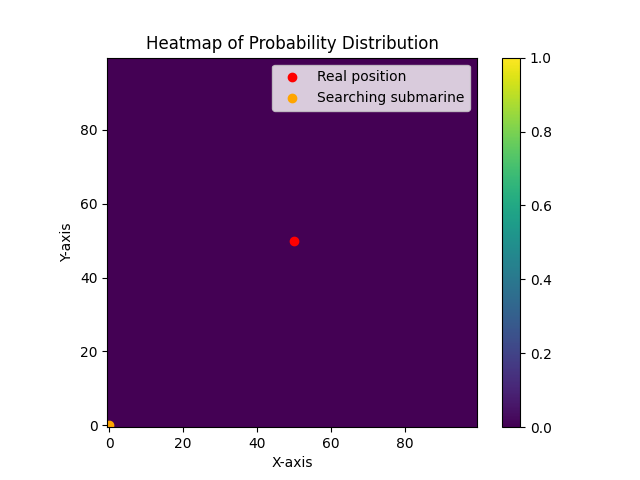
\includegraphics[width=0.7\textwidth]{0-xy.png}
\caption{Generation at The Beginning}
\label{fig:re1}
\end{figure}

We can see in Figure \ref{fig:re1} that at the beginning, the searching submarine is at the edge of the grid. Because the position of the submersible is determined at the beginning, so there is only one region with a probability of 1. For all the other regions, the probability is zero. The reason why the whole plane seems to be of probability zero is that the region where the probability is 1 is blocked by the red dot that represents the current position of the submersible.
\begin{figure}[H]
  \begin{minipage}{0.5\textwidth} % 设置图片占据页面宽度的一半
    \centering
    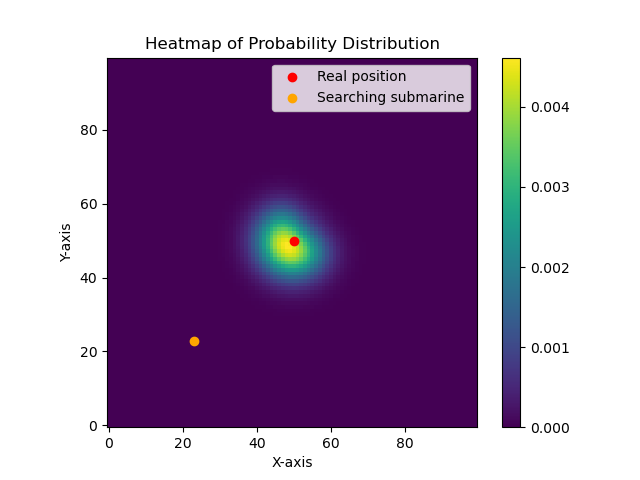
\includegraphics[width=\linewidth]{xy.png}
    \caption{Generation after Some Time: xy}
    \label{fig:re2}
  \end{minipage}
  \begin{minipage}{0.5\textwidth} % 设置图片占据页面宽度的一半
    \centering
    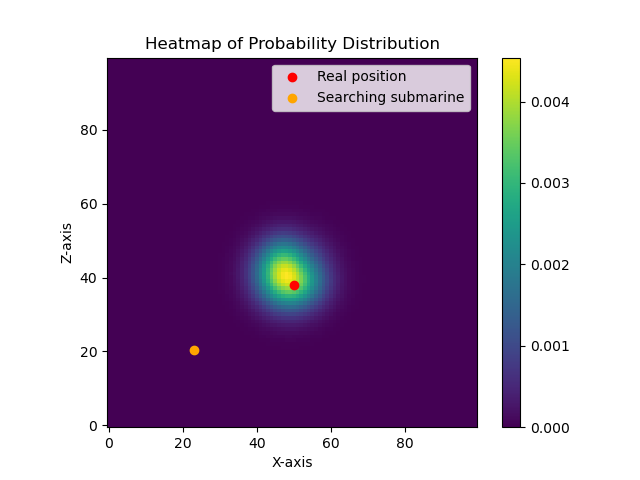
\includegraphics[width=\linewidth]{xz.png}
    \caption{Generation after Some Time: xz}
    \label{fig:re2.5}
  \end{minipage}
\end{figure}

In Figures \ref{fig:re2} and \ref{fig:re2.5}, we can see that after a few seconds, the probability distribution has spread out, but the real position is still not far from the regions where probability is highest. Meanwhile, the searching submarine has been moving steadily towards the submersible's real position. This can be seen on both the xy and xz planes.


\begin{figure}[H]
\centering
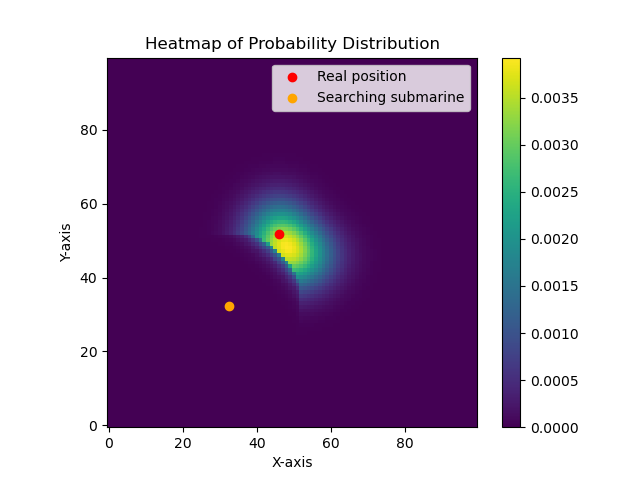
\includegraphics[width=0.7\textwidth]{ecipse.png}
\caption{Generation When the Accumulated Search Results Intervened}
\label{fig:re5}
\end{figure}

The distribution shown in figure \ref{fig:re5} looks sort of like an eclipse. This is because when the searching submarine did not find the submersible in regions with probability greater than zero, we updated the probability distribution based on this result. It's like we carve a sphere out of the probability distribution after every failed search. Note that the real position is still not far from the regions where probability is highest.

\section{Strengths and Weaknesses}
\subsection{Our Strengths}
\begin{enumerate}[\bfseries 1.]
    \setlength{\parsep}{0ex} %段落间距
    \setlength{\topsep}{0.5pt} %列表到上下文的垂直距离
    \setlength{\itemsep}{0.5pt} %条目间距
    \item \textbf{Rationality and Authenticity} Our model takes many factors into account. It's factual and reasonable. Our model considers the different density of water, impact of currents, geography of sea floor, probability of propulsion loss, and utilizes the accumulated searching results. 
    \item \textbf{Realizability} The data our model need can be either accessed online or accurately computed, as is demonstrated in the \textbf{Model Preparation} section. Our model can be implemented with code, as is shown in the \textbf{Model Implementation} section. 
    \item \textbf{Accuracy} Our model can accurately and quickly predict the position of the lost submersible. As we have taken many factors into account, our model is accurate enough to help rescue the lost submersible.
    \item  \textbf{Flexibility and Extensibility} Our model can be extended from Ionian Sea to other areas easily. All you need to do is to get the deserved data of the target area.
\end{enumerate}
\subsection{Our Weaknesses}
\begin{enumerate}[\bfseries 1.]
    \setlength{\parsep}{0ex}
    \setlength{\topsep}{0.5pt}
    \setlength{\itemsep}{0.5pt}
    \item \textbf{Complexity} Our model has many redundant computations. As is shown in the figure in \textbf{Model Implementation} section, there are a large number of regions whose probability densities are all zero, which will result in redundant computations.
    \item \textbf{Overly Detailed} Our model is overly detailed in certain details that may not be very important. That will increase the computation burden.
\end{enumerate}
\section{Future Work}
As mentioned in the section of our weaknesses, there is still room for improvement for our model. To begin with, although we realize the need for computation speed and set out to shorten the speed of our model, we still need much time for our calculations. In an emergency situation where every second counts, the model should be as fast as possible. Perhaps the use of certain data structures and algorithms can further shorten the computation time.

Next, \textbf{the initial position} of the searching submarine may deserve further consideration. In our model, we assume the initial position is (0,0,0), but if we take the actual place of the sunken shipwreck to be visited into account, maybe we can find a place both at shore and at a closer distance for the searching submarine to wait for orders. However, due to the fact that we do not possess this data when solving the problem, we simply assumed the initial position to be (0,0,0).

Finally, as stated in the \textbf{Extrapolate} section, there may be multiple submersibles in the same vicinity in the future. If more than one submersible needs to be rescued, our current approach is to send out multiple searching submarines, duplicating the location and search process of rescuing only one submersible. However, because the submersibles were originally in the same vicinity, this approach may result in the searching submarines clogging up, wasting detection space. Perhaps a more efficient approach will be to scatter the searching submarines a bit, at least making sure that their detection space does not coincide too much. This calls for the need of another model, but due to the limited time, we can only present our idea here.
\clearpage   %另起一页继续写。
\begin{letter}{Memo}
\begin{flushleft}  % 左对齐环境,无首行缩进
\textbf{To:} The Greek Government\\
\textbf{From:} MCM Team \#2419335 \\
\textbf{Date:} February 6th, 2024\\
\textbf{Subject:} Probability-Based Rescue Model for Submersibles
\rule{\linewidth}{2pt}
\end{flushleft}
\noindent{Your Excellency:}

In recent years, business activities about exploring are getting more and more popular. After the equipment of great detect devices, how to ensure the safety of the submersible becomes an urgent issue. Our team has developed a widely applicable model to achieve the purpose of minimizing the time to find the lost submersible. We appreciate the opportunity to introduce our strategy to you. 

Considering the reaction of people staying in the submersible, the wisest choice for the captain is to go straight up, as the host ship know its current coordinate. Thus, the captain of the host ship can minimize the probable activity radius of the lost submersible and reduce the difficulty of finding it.

With this prerequisite, we can predict the most likely location of the lost submersible over time. When we provide data such as the depth, temperature, salinity, and the current speed of ocean currents at various points of the Ionian Sea, we can obtain from the model the most probable location of the submersible every second. Since the searching submarine scans the surrounding sea area continuously from the starting point, we can constantly update the heat map of the possible location of the submersible. The host ship always moves towards the average position weighed by probability on the current heat map. As our model employs a dynamic programming algorithm, we can continuously adjust the current optimal plan to ensure that the searching submarine does not blindly head towards locations with a lower probability, wasting precious rescue time.

\begin{figure}[H]
\centering
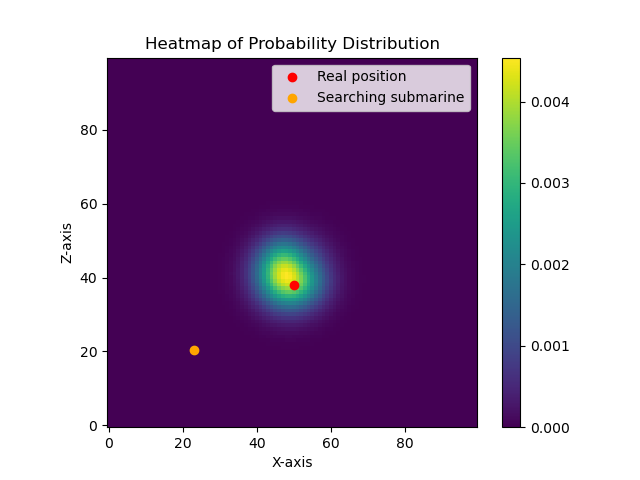
\includegraphics[width=0.7\textwidth]{memofirst.png}
\caption{First Heat Map}
%\label{fig:re5}
\end{figure}
In the first image, the real position of the missing submersible can be clearly seen near the center of the bright spot, indicating that our direction towards the center of the bright spot at this moment is accurate. Considering the radar's detection radius, we can almost ascertain the position of the missing submersible directly when the ship arrives near the center of the bright spot.

\begin{figure}[H]
\centering
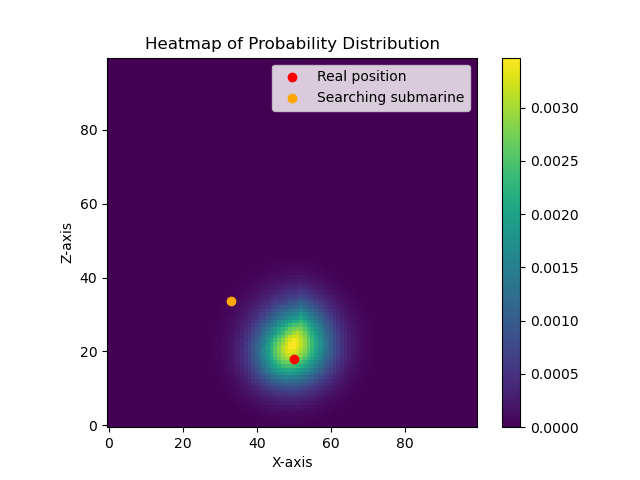
\includegraphics[width=0.7\textwidth]{memosecond.png}
\caption{Second Heat Map}
%\label{fig:re5}
\end{figure}
In the second image, the actual position is still locked near the center of the bright spot, which once again proves the rationality of our execution strategy. As seen, compared to the first image, the position of the bright spot has changed significantly. At this time, the dynamic programming algorithm allows us to adjust the route in time, turn around, and continue moving towards the red dot, shortening the search time.

Considering the urgency, timeliness of rescue, comprehensiveness of detection and cost of equipment, we recommend that ships conducting detection in the Ionian Sea use software with our model as the core to determine the position of the submersible based on real-time ocean data, search and rescue directions and other strategies. We are eager to help you ensure the safety of every submersible. If you have any further questions about our solution, please feel free to contact us. Our team members are willing to solve any questions you have and renew our model.

Hope we can keep cooperating.

\begin{flushright}
Yours sincerely

Team: \#2419335
\end{flushright}

\end{letter}

% 参考文献
\clearpage
\begin{thebibliography}{99}
    \bibitem{Titanic tourist submersible} Titanic tourist submersible: desperate search for sub missing with five onboard, The Guardian, https://www.theguardian.com/uk-news/2023/jun/19/titanic-tourist-submarine-missing-north-atlantic
    \bibitem{Ionian Sea Research} Knutsen, Øyvind, Stefanakos, Christos, and Dag Slagstad. "Ocean current conditions in the Ionian Sea." Paper presented at the The 31st International Ocean and Polar Engineering Conference, Rhodes, Greece, June 2021.
    \bibitem{Blue-greenway} BLUE-GREENWAY: Ocean current conditions in the Ionian Sea, Regional Funds Online Magazine, https://regionalcoopmag.net/2021/08/22/blue-greenway-ocean-current-conditions-in-the-ionian-sea/
    \bibitem{Weibull Distribution} Weibull distribution, Wikipedia, https://en.wikipedia.org/wiki/Weibull\_distribution
    \bibitem{TEOS-10} TEOS-10, Wikipedia, https://en.wikipedia.org/wiki/TEOS-10
    \bibitem{communication methods} How Do Submarines Communicate, Maritime page, https://maritimepage.com/how-do-submarines-communicate/

\end{thebibliography}


\end{document}